\documentclass[12pt,a4paper]{article}
\usepackage[top=2.7cm, bottom=2cm, left=2cm, right=2cm]{geometry}
\usepackage[utf8]{inputenc}
\usepackage{CJKutf8}
\usepackage{enumitem}
\usepackage{verbatim}


%% Useful packages
\usepackage{amsmath,amssymb}
% \usepackage{subfigure}
\usepackage{graphicx,wrapfig}
\usepackage[dvipsnames,table]{xcolor}
\usepackage[table]{xcolor}
\usepackage{url}
\usepackage{setspace}
\usepackage[colorlinks=true,anchorcolor=black,linkcolor=Blue,urlcolor=RoyalBlue]{hyperref}
\usepackage[linesnumbered,ruled,vlined]{algorithm2e}
\usepackage{threeparttable}

\usepackage{tikz}
\usepackage{blindtext}
\usepackage{titlesec}
\usepackage{courier}
\usepackage{pdfpages}

\usepackage{lastpage}
\usepackage{fancyhdr}
\setlength{\headheight}{0pt}
\renewcommand{\headrulewidth}{1pt} % remove lines
\renewcommand{\footrulewidth}{0pt}
\pagestyle{fancyplain}
\fancyhf{}
\lhead{
  \textcolor{Gray}{Group 2}
}
\rhead{
  \begin{CJK}{UTF8}{bkai}
  \textcolor{Gray}{實驗物理學實驗結報}
  \end{CJK}
}
\lfoot{
   \textcolor{Gray}{March 4}
  }
\rfoot{
  \thepage/\pageref{LastPage}
  }

\title{\vspace{-0.5cm}
       {\bf \textcolor{black}{{\LARGE 
       \begin{CJK}{UTF8}{bkai}
       實驗物理學(二)\\
       \vspace{6pt}
       實驗紀錄\\
       \vspace{60pt}
       實驗二、阻抗 Impedance
       \end{CJK}
       }}
       }
       }
\author{}
\date{}

\begin{document}
\begin{CJK}{UTF8}{bkai}

\maketitle
\thispagestyle{empty}

\vspace{10cm}
\begin{center}
{\large 第二組}\\ \vspace{12pt}
{\large \makebox[3em][s]{洪\hspace{\fill}瑜} B125090009}\\ \vspace{6pt}
{\large \makebox[3em][s]{黃巧涵}  B122030003}\\ \vspace{6pt}
{\large \makebox[3em][s]{洪懌平} B102030019}\\ \vspace{12pt}
{\large 2025/03/04}\\
\end{center}

\clearpage

\section{實驗目的}

\begin{enumerate}
    \item 近一步實作量測儀器本身的輸出與輸入阻抗
    \item 認識戴維寧等效電路
    \item 認識及實際應用奈奎斯特取樣定理與混疊
\end{enumerate}


\section{實驗原理}
\subsection{阻抗}
\hfill

阻抗$Z$是交流電路中對電流的總反抗能力,但同時包含電阻、電感、電容的綜合效應。它是一個複數數量,包含實部 (電阻 $R$) 和虛部 (電抗$X$),可表示為:
\begin{equation*}
    Z = R + jX
\end{equation*}
$X$又分成:
\begin{itemize}
    \item 感抗 $X_{L}$: $X_{L} = \omega L$
    \item 容抗 $X_{C}$: $X_{C} = 1/\omega C$
\end{itemize}

而電阻、電容、電感的阻抗可表示為:

\begin{itemize}
    \item 電阻: $Z_{R} = R$
    \item 電容: $Z_{C} = \frac{1}{j\omega C}$
    \item 電感: $Z_{L} = j\omega L$
\end{itemize}

\subsection{三用電錶的電壓檔 AC與DC響應現象}
\hfill

頻率響應現象指的是系統對不同頻率的輸入訊號產生不同的輸出。
在三用電表中:
\begin{itemize}
    \item DCV (直流電壓檔):\\
    主要測量直流電壓,內部有低通濾波器,會衰減高頻 AC 訊號,因此測量 AC 電壓時不準確。
    \item ACV (交流電壓檔):\\
    透過整流和濾波電路測量 AC 訊號的 RMS 值,但因為整流器、濾波器和內部放大器的 頻率響應不同,對不同頻率的 AC 訊號可能產生誤差。
\end{itemize}

這就是三用電表的 AC 和 DC 量測會有頻率依賴性響應的原因

\subsection{戴維寧等效電路}
\hfill

戴維寧等效電路是一種簡化電路的方法,用以下表示:

任何線性電路可以用一個獨立電壓源Vth(戴維寧電壓源)和一個電阻二端網絡的串聯電阻(也就是戴維寧等效電阻Rth)組合來等效。在單頻交流系統中,此定理不僅適用於電阻,也適用於廣義的阻抗;可方便計算負載上的電壓和電流
\begin{itemize}
    \item $V_{th}$:輸出端開路時測得電壓
    \item $R_{th}$:將所有獨立電壓源短路、電流源開路後,從輸出端看入的等效電阻
\end{itemize}

\subsection{DAQ card(Data Acquisition Card)}
\hfill

DAQ (資料擷取) 卡:
\begin{itemize}
    \item \textbf{AI (Analog Input; 類比輸入):}用來讀取外部類比訊號,例如感測器輸出的電壓訊號。輸入範圍受限於 DAQ 卡的規格 (如$\pm$10V)
    \item \textbf{AO (Analog Output; 類比輸出):}產生類比訊號,例如控制電壓輸出(通常範圍也是$\pm$10V)
    \item \textbf{DI (Digital Input; 數位輸入):}讀取數位訊號 (0 或 1)
    \item \textbf{DO (Digital Output; 數位輸出):}輸出數位訊號,例如控制開關或 LED
    \item \textbf{GND (接地):}提供參考電位

\end{itemize}

\subsection{奈奎斯特取樣定理與混疊 (aliasing effect)}\label{subsec:ny}
\hfill

\begin{itemize}
    \item 奈奎斯特取樣定理(Nyquist Sampling Theorem):\\
    訊號處理中,若要正確重建一個頻率最高為 fmax 的類比訊號,取樣頻率 fs必須至少是該頻率的兩倍,i.e.,
    \begin{equation*}
    f_{s} \ge 2f_{max}
    \end{equation*}
    奈奎斯特取樣定理是避免混疊的必要條件
    \item 混疊 (aliasing effect):\\
    取樣後訊號的頻率重疊,就是高於取樣頻率一半的頻率成分將被重建成低於取樣頻率一半的訊號。這種頻譜的重疊導致的失真稱為混疊;結合剛剛的奈奎斯特取樣定理,如果取樣頻率低於奈奎斯特頻率,則高頻訊號會錯誤地映射到較低頻率,造成失真。
\end{itemize}


\clearpage
\section{實驗步驟}

\subsection{練習一:歐姆檔的輸出阻抗}\label{subsec:step_1}
\hfill

\textbf{“請同學根據第一次實驗的結果,選擇適當的電阻R,畫出歐姆檔每一個檔位的戴維寧等效電路。”}

\begin{figure}[h]
    \centering
    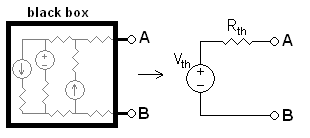
\includegraphics[width=0.6\linewidth]{figures/Thevenin_equivalent.png}
    \caption{戴維寧電路示意圖(credit:Wikipedia 戴維寧定理; 參考資料[1])}
    \label{fig:thevenin}
\end{figure}



\subsection{練習二:訊號產生器的輸出阻抗}\label{subsec:step_2}
\hfill

\textbf{“下圖為訊號產生器的輸出阻抗的量測電路圖,利用示波器觀察開路情況下($R_{L}$不接)的訊號,調整使其振幅為 200 mV,頻率 1 kHz,OFFSET 為 0 之弦波訊號。 然後 RL分別換成 47、100、220、470$\Omega$電阻 (這些電阻請事先用電表之歐姆檔測量並記錄其值),記錄$V_{out}$,由負載效應求出$R_{S}$”}


\begin{figure}[h]
    \centering
    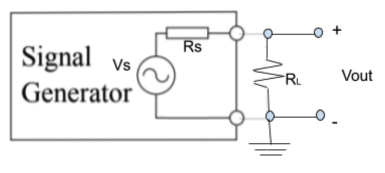
\includegraphics[width=0.5\linewidth, angle=0]{figures/exp_2.png}\\
    \includegraphics[width=0.5\linewidth, angle=0]{figures/PXL_20250304_065300968.MP.pdf}
    \caption{練習二線路示意圖(上; credit:實驗講義)和實際操作架設圖(下)}
    \label{fig:exp_4}
\end{figure}




\clearpage
\subsection{練習三:測量示波器的輸入阻抗(一般檔 $\times$1 檔)}\label{subsec:step_3}
\hfill

\textbf{“利用下圖之分壓器電路圖,$V_{in}$輸入100 Hz, $V_{pp}$= 10 V (DC OFFSET = 0)之正弦函數信號,用示波器看$V_{out}$,這裡探針調在 X1 檔,$R_{1}$和$R_{2}$用1k、100 k、1M及10M$\Omega$不同值之電阻分別代替,紀錄 Vout 的變化。不同電阻值的分壓器,結果有何不同? 計算出示波器的輸入阻抗。”}

\begin{figure}[h]
    \centering
    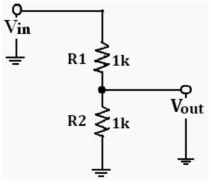
\includegraphics[width=0.3\linewidth]{figures/exp_3.png}\\
    \includegraphics[width=0.5\linewidth]{figures/PXL_20250304_072434229.pdf}
    \caption{練習三線路示意圖(上; credit:實驗講義)和實際操作架設圖(下)}
    \label{fig:exp_3}
\end{figure}


% \clearpage
\subsection{練習四:數據擷取:將類比輸入波形轉換為數位資料}\label{subsec:step_4}
\hfill

\textbf{利用DAQ卡擷取訊號產生器的訊號}

\begin{figure}[h]
    \centering
    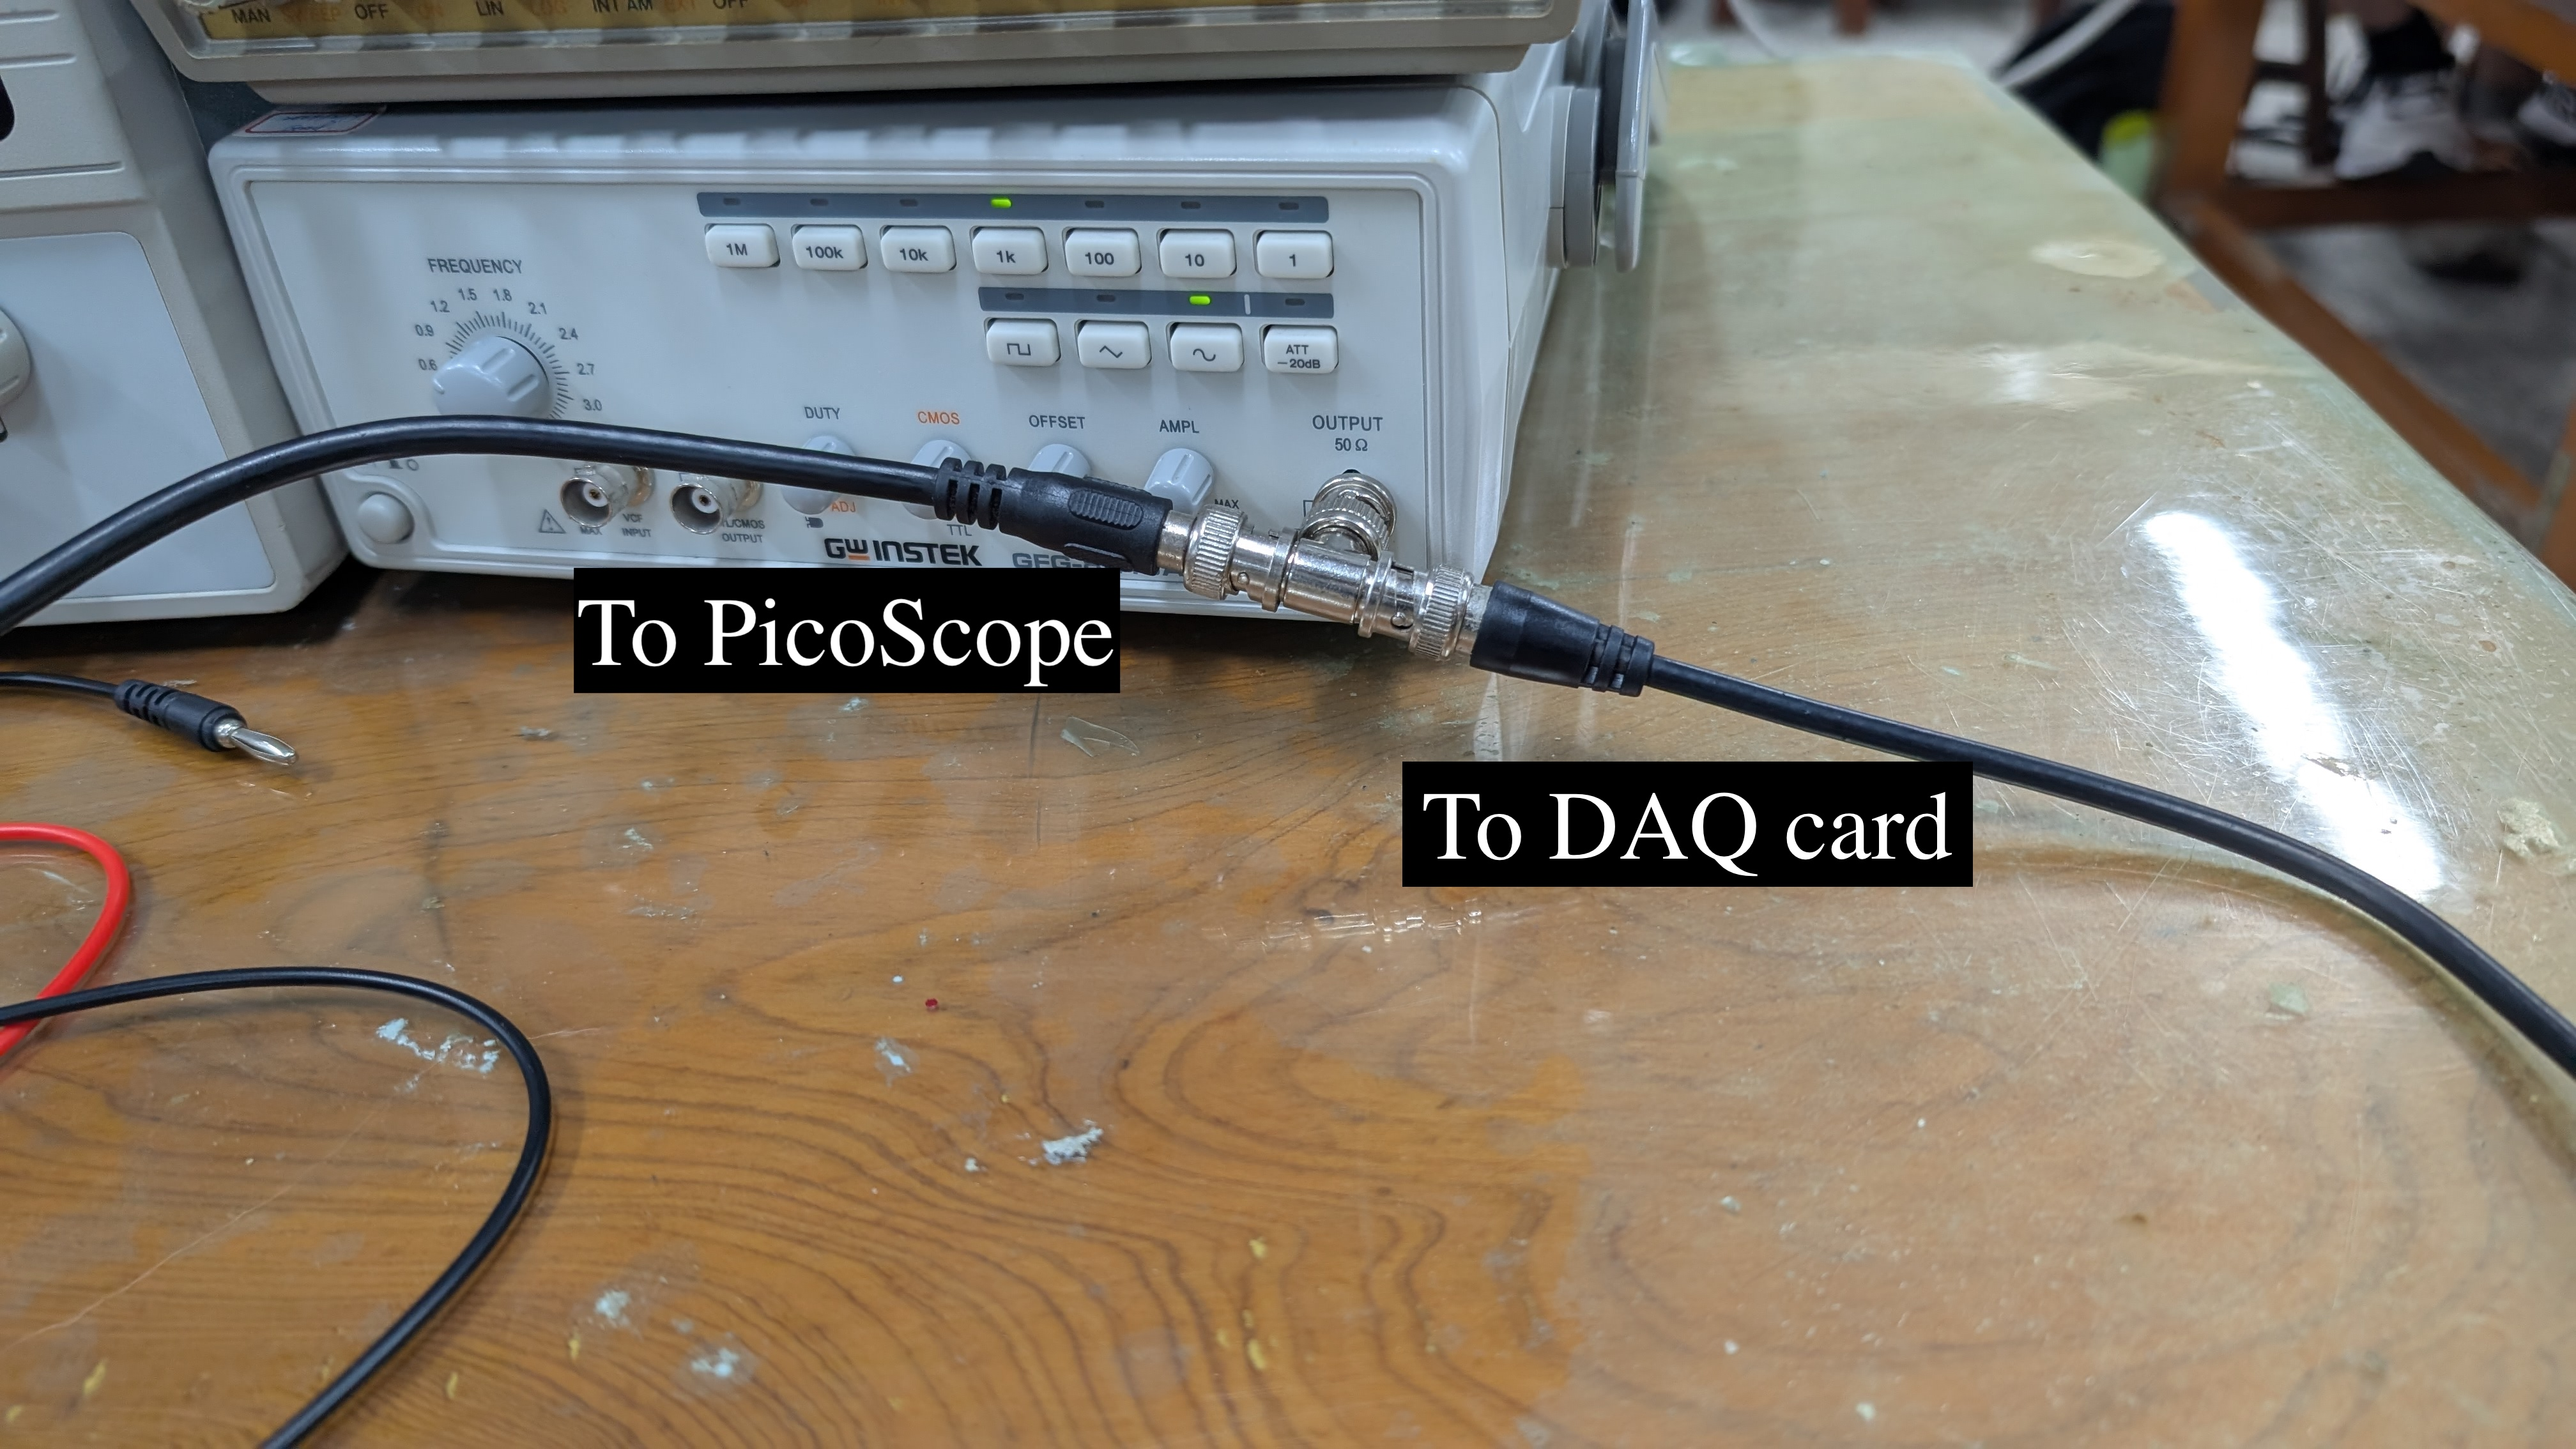
\includegraphics[width=0.5\linewidth]{figures/exp_4.jpg}
    \caption{練習四實際操作線路}
    \label{fig:exp_4}
\end{figure}


\clearpage
\section{實驗數據}

\subsection{練習一:歐姆檔的輸出阻抗}
\hfill

根據第一次之實驗結果,結合公式:
\begin{equation}
\label{eq:va_rout}
    V_{out} = V_{th} \frac{R_{x}}{R_{th}+R_{x}}
\end{equation}
可推算出下列結果:

\begin{center}
    \begin{tabular}{c|c|c}
    \multicolumn{3}{c}{三用電表、三用電表和$R_{x}=$10.2$\Omega$(理論10$\Omega$)的電阻串聯}\\
    \hline
    \hline
    $\Omega$檔位  &  內部電壓$V_{th}$(V)   &   內部等效電阻
    $R_{th}$($\Omega$)\\
    \hline
    \hline
    20M &   $<$0.00   &   $\sim\infty$\\\hline
    200k    &   $<$0.00    &   $\sim\infty$\\\hline
    20k    &   0.03    &   $\sim\infty$\\\hline
    2k    &   1.00    &   7.39\\\hline
    200    &   1.20    &   5.10\\\hline
    \end{tabular}
\end{center}

\begin{center}
    \begin{tabular}{c|c|c}
    \multicolumn{3}{c}{三用電表、三用電表和$R_{x}=$997$\Omega$(理論1k$\Omega$)的電阻串聯}\\
    \hline
    \hline
    $\Omega$檔位  &  內部電壓$V_{th}$(V)   &   內部等效電阻
    $R_{th}$($\Omega$)\\
    \hline
    \hline
    20M &   $<$0.00    &   $\sim\infty$\\\hline
    200k    &   3.80   &   120.94\\\hline
    20k    &   28.80   &   14.44\\\hline
    2k    &   83.20   &   5.07\\\hline
    200    &   102.40    &   $<$0.00\\\hline
    \end{tabular}
\end{center}

\subsection{練習二:訊號產生器的輸出阻抗}
\hfill

\begin{center}
\begin{tabular}{c|c|c}
    \multicolumn{3}{c}{練習二實驗數據}\\\hline
    $R_{L}$($\Omega$)   &   $V_{out}$(V)    &   $R_{S}$($\Omega$)\\
    \hline\hline
    47  &   21  &   422.55  \\\hline
    100 &   29  &   623.45  \\\hline
    220 &   36  &   1062.11 \\\hline
    470 &   42  &   1877.76 \\\hline
\end{tabular}
\end{center}

\subsection{練習三:測量示波器的輸入阻抗(一般檔 $\times$1 檔)}
\hfill

\begin{center}
\begin{tabular}{c|c}
\multicolumn{2}{c}{練習三實驗數據}\\
\hline
$R_{1}, R_{2}$($\Omega$)    &   $V_{out}$(V)\\
\hline
\hline
1k  &   4.54\\\hline
10k &   4.92\\\hline
100k    &   4.71\\\hline
1M &   3.36\\\hline
10M  &   0.87\\\hline
\end{tabular}
\end{center}

\clearpage

\subsection{練習四:數據擷取:將類比輸入波形轉換為數位資料}
\hfill

\begin{figure}[h]
    \centering
    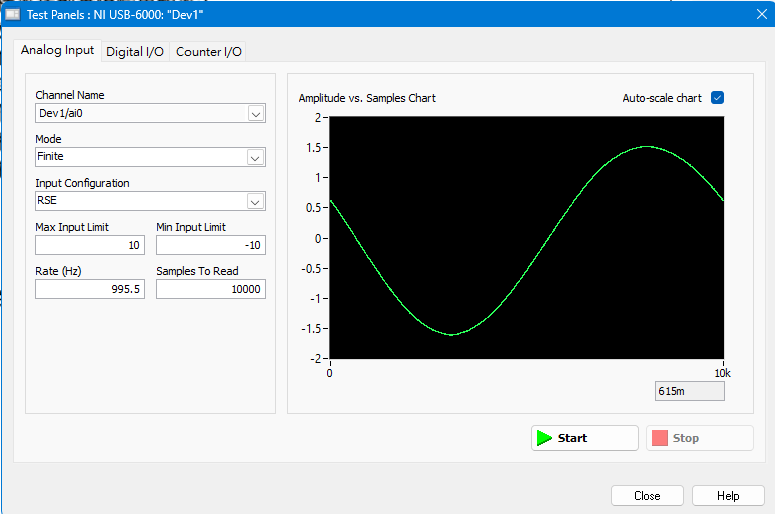
\includegraphics[width=0.7\linewidth]{figures/1_995_995.png}
    \caption{訊號產生器頻率$f_{in}$=995.5Hz,取樣頻率$f_{s}$=995.5Hz}
    \label{fig:exp_4_1}
\end{figure}

\begin{figure}[h]
    \centering
    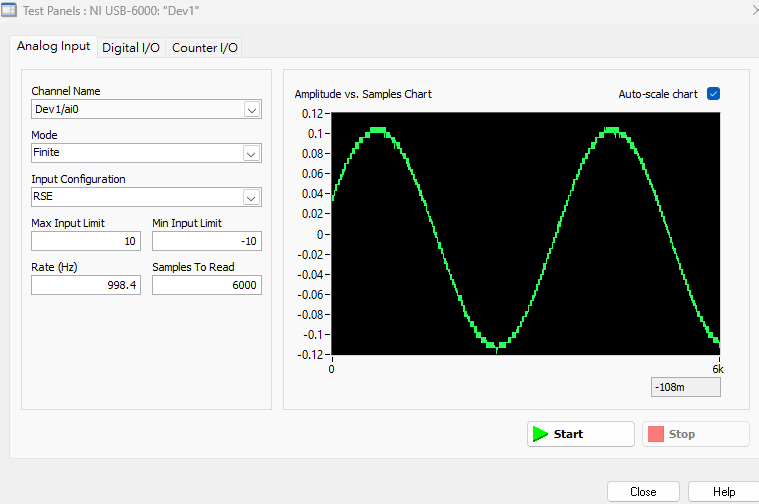
\includegraphics[width=0.7\linewidth]{figures/2_999.4_998.4.png}
    \caption{訊號產生器頻率$f_{in}$=999.4Hz,取樣頻率$f_{s}$=998.4Hz}
    \label{fig:exp_4_2}
\end{figure}
\clearpage

\begin{figure}[h]
    \centering
    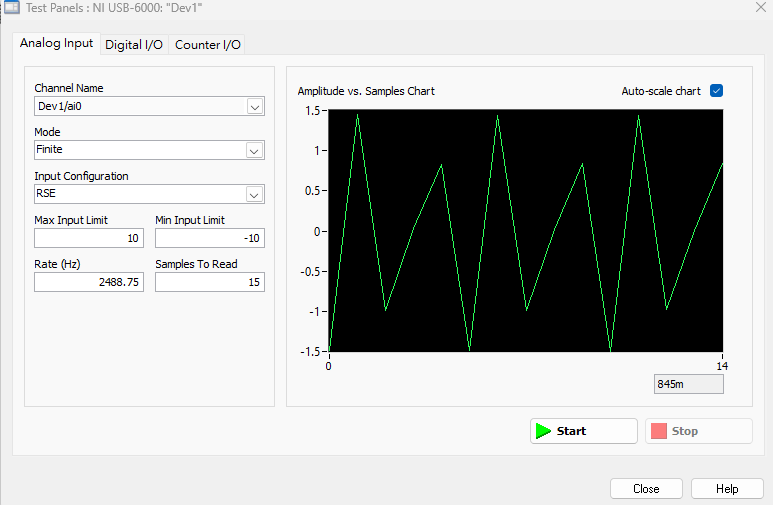
\includegraphics[width=0.7\linewidth]{figures/exp_4_3.png}
    \caption{訊號產生器頻率$f_{in}$=995.5Hz,取樣頻率$f_{s}$=2,488.75Hz}
    \label{fig:exp_4_3}
\end{figure}

\begin{figure}[h]
    \centering
    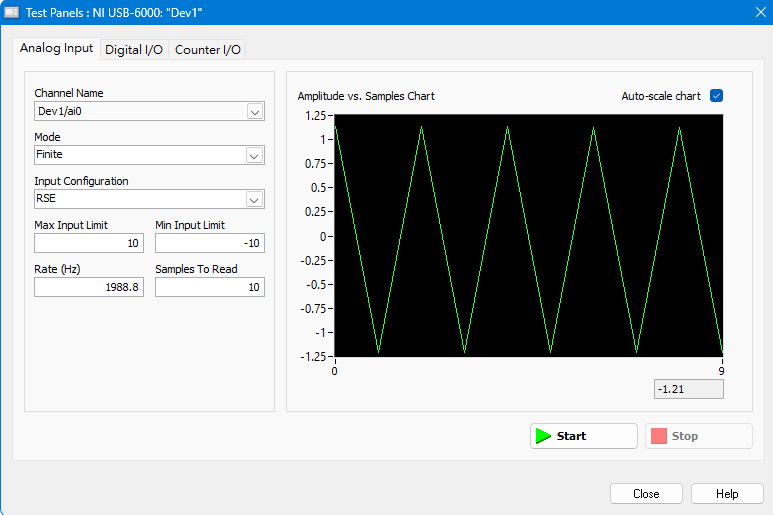
\includegraphics[width=0.7\linewidth]{figures/exp_4_4_1.png}
    \caption{訊號產生器頻率$f_{in}$=994.5Hz,取樣頻率$f_{s}$=1988.8Hz(2倍)}
    \label{fig:exp_4_4_1}
\end{figure}
\clearpage

\begin{figure}[h]
    \centering
    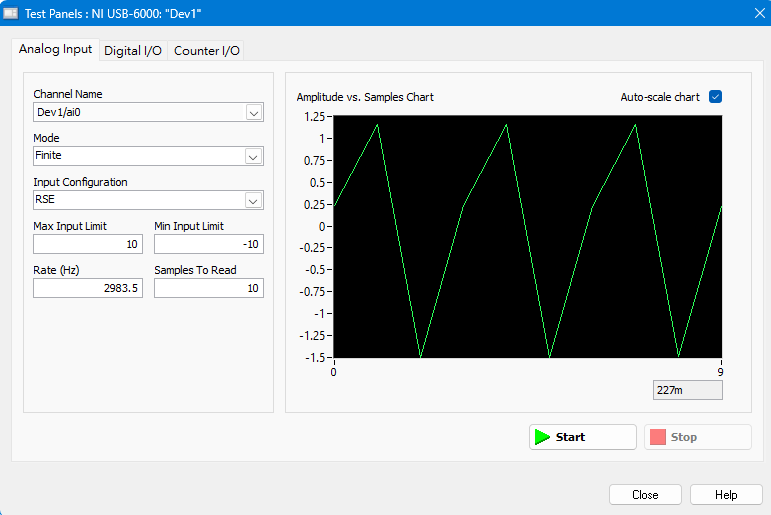
\includegraphics[width=0.7\linewidth]{figures/exp_4_4_2.png}
    \caption{訊號產生器頻率$f_{in}$=994.5Hz,取樣頻率$f_{s}$=2983.5Hz(3倍)}
    \label{fig:exp_4_4_2}
\end{figure}

\begin{figure}[h]
    \centering
    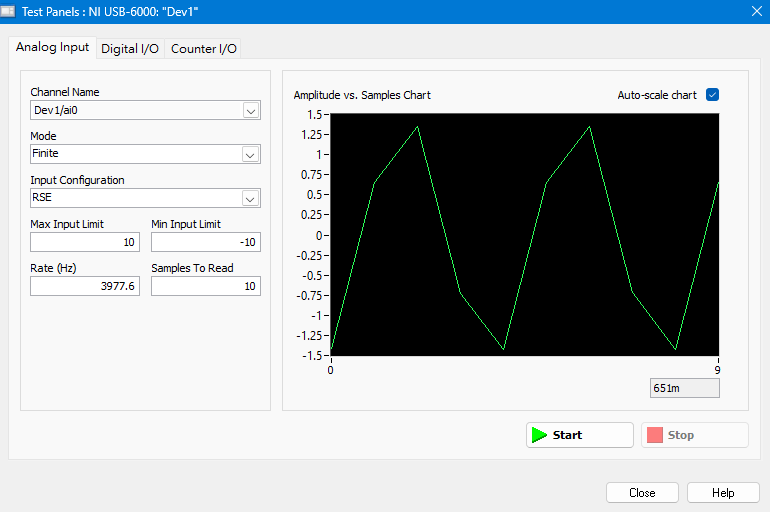
\includegraphics[width=0.7\linewidth]{figures/exp_4_4_3.png}
    \caption{訊號產生器頻率$f_{in}$=994.5Hz,取樣頻率$f_{s}$=3977.6Hz(4倍)}
    \label{fig:exp_4_4_3}
\end{figure}
\clearpage

\begin{figure}[h]
    \centering
    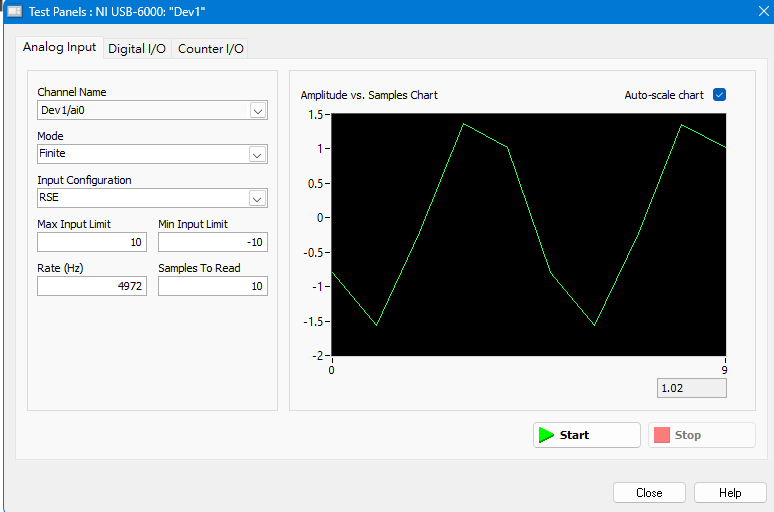
\includegraphics[width=0.7\linewidth]{figures/exp_4_4_4.png}
    \caption{訊號產生器頻率$f_{in}$=994.5Hz,取樣頻率$f_{s}$=4972Hz(5倍)}
    \label{fig:exp_4_4_4}
\end{figure}

\begin{figure}[h]
    \centering
    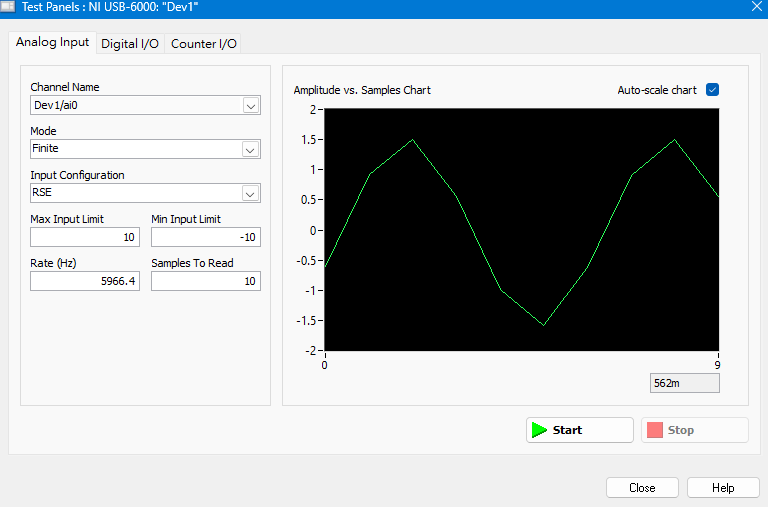
\includegraphics[width=0.7\linewidth]{figures/exp_4_4_5.png}
    \caption{訊號產生器頻率$f_{in}$=994.5Hz,取樣頻率$f_{s}$=5966.4Hz(6倍)}
    \label{fig:exp_4_4_5}
\end{figure}
\clearpage

\begin{figure}[h]
    \centering
    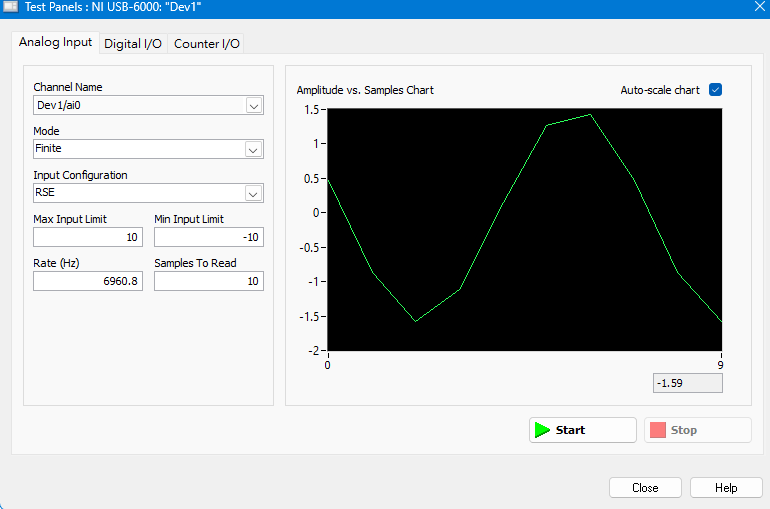
\includegraphics[width=0.7\linewidth]{figures/exp_4_4_6.png}
    \caption{訊號產生器頻率$f_{in}$=994.5Hz,取樣頻率$f_{s}$=6960.8Hz(7倍)}
    \label{fig:exp_4_4_6}
\end{figure}

\clearpage
\section{實驗分析和問題討論}

\subsection{練習一:歐姆檔的輸出阻抗}
\hfill

\begin{itemize}
    \item 戴維寧等效電壓$V_{th}$:即為表格中「內部電壓$V_a$」;表示三用電表在該檔位時對外部電阻(997$\Omega$)提供的開路電壓。
    \item 戴維寧等效電阻$R_{th}$:即為表格中「內部等效電阻$R_{out}$」;表示三用電表在該檔位的輸出阻抗。
\end{itemize}

外部電阻選擇997歐姆,而非10.2歐姆;主要因素為:
負載電阻小導致負載電壓下降:從戴維寧等效電路來看,負載電壓(V)由三用電表內部等效電阻($R_{th}$)和外部負載電阻(R)組成的分壓電路決定

\begin{equation*}
V=V_{th} \frac{R}{R_{th}+R}
\end{equation*}

因此,可畫出歐姆檔每一個檔位的戴維寧等效電路(如Fig.\ref{fig:thevenin}; 參考資料[2])
\begin{itemize}
    \item 20M$\Omega$檔位:\\
    \begin{figure}[h]
        \centering
        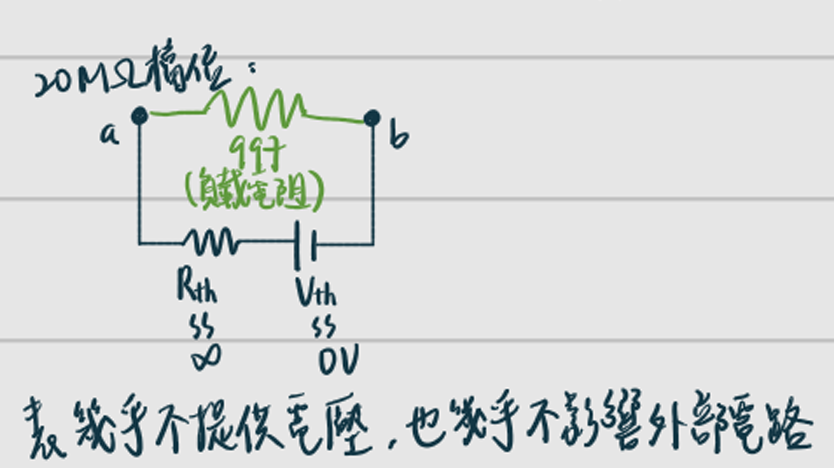
\includegraphics[width=0.5\linewidth]{figures/20M.png}
        \caption{20M$\Omega$檔位}
        \label{fig:20m}
    \end{figure}
    \item 200k$\Omega$檔位:\\
    \begin{figure}[h]
        \centering
        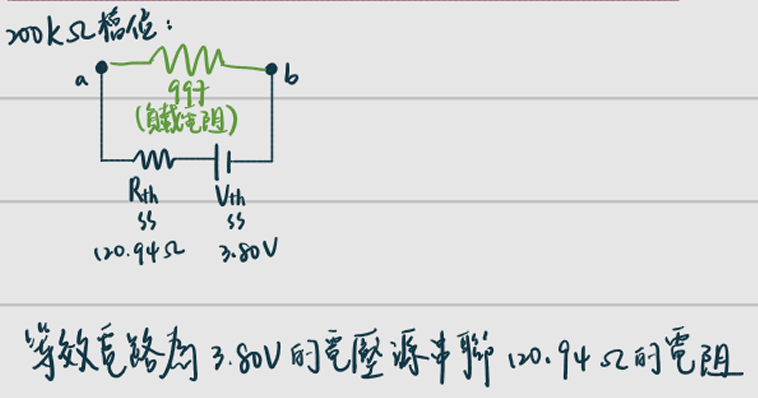
\includegraphics[width=0.5\linewidth]{figures/200k.png}
        \caption{200k$\Omega$檔位}
        \label{fig:200k}
    \end{figure}
    \clearpage
    \item 20k$\Omega$檔位:\\
    \begin{figure}[h]
        \centering
        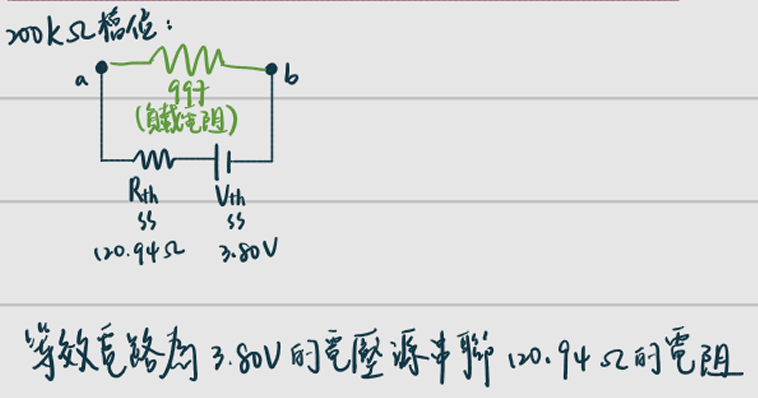
\includegraphics[width=0.5\linewidth]{figures/20k.png}
        \caption{20k$\Omega$檔位}
        \label{fig:20k}
    \end{figure}
    \item 2k$\Omega$檔位:\\
    \begin{figure}[h]
        \centering
        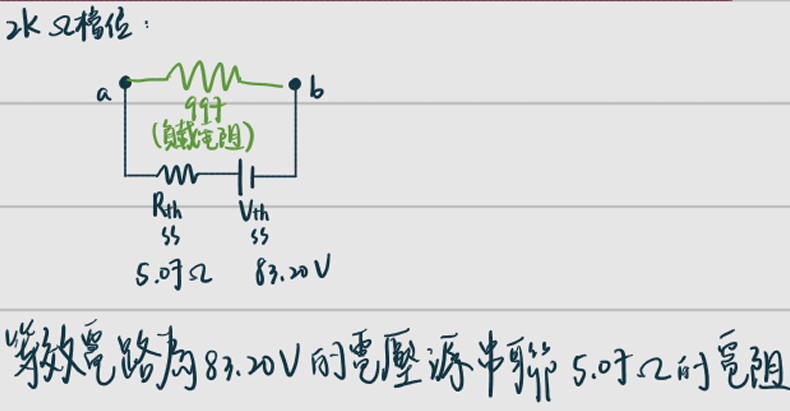
\includegraphics[width=0.5\linewidth]{figures/2k.png}
        \caption{2k$\Omega$檔位}
        \label{fig:20k}
    \end{figure}
    \item 200$\Omega$檔位:\\
    \begin{figure}[h]
        \centering
        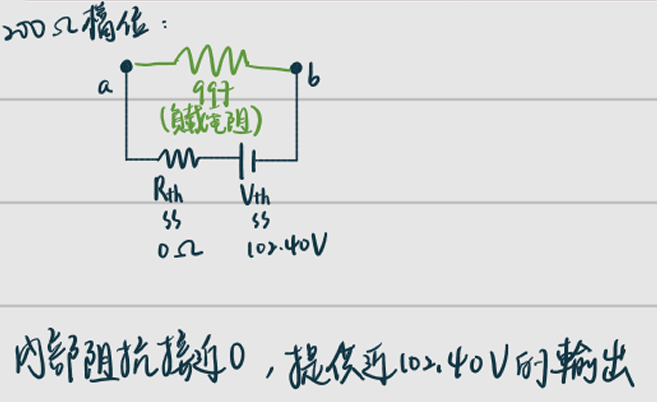
\includegraphics[width=0.5\linewidth]{figures/200.png}
        \caption{200$\Omega$檔位}
        \label{fig:200}
    \end{figure}
\end{itemize}

\subsection{練習二:訊號產生器的輸出阻抗}
\hfill

使用分壓公式:
\begin{equation*}
V_{out}=V_{open}\frac{R_{L}}{R_{s}+R_{L}}
\end{equation*}
將此式改寫為:
\begin{equation*}
R_{s}=R_{L} \left( \frac{V_{open}}{V_{out}}-1\right)
\end{equation*}
可以推算出數值$R_{s}$。

由實驗數據表格可看出,隨著電阻值增加,$V_{out}$與$R_s$皆有上升的趨勢。
透過觀察分壓公式可以看出,當$R_L$值上升,會就使得$V_{out}$數值上升,符合我們從實驗得出的數據;然而在Rs數值的部分,訊號產生器之內電阻應為一固定之數值,而本次實驗所使用之訊號產生器型號為GFG-8215A,經查詢其產品規格書,發現規格書上標記訊號產生器之內電阻為50Ω±10\%,而實驗結果平均值卻為1011.52Ω,規格書與實驗結果推算出之數值有落差。

推斷誤差來源可能有:
\begin{enumerate}
    \item 測量時使用的三用電表由於頻率響應,導致測得數值出現誤差
    \item 商品規格書標示之阻抗數值與實際情形不符
\end{enumerate}
由於訊號產生器輸出之訊號由示波器監控,確認該訊號$V_{open}$數值無誤,因此我們認為$V_{open}$不是其中一個導致誤差產生的原因。此外電阻的實際數值也都在實驗開始前進行量測,確保計算時使用的電阻數值正確,因此電阻也不是其中一個導致誤差產生的原因。


\subsection{練習三:測量示波器的輸入阻抗(一般檔 $\times$1 檔)}
\hfill

根據公式:
\begin{equation*}
    V_{out}=V_{in}\frac{R_2}{R_1+R_2+Z_{in}}
\end{equation*}

本實驗使用PicoScope軟體模擬示波器,而與使用硬體示波器應測量出的趨勢並不相同。理論上,根據實驗一的結果討論,選擇$R_1=R_2$時,可知應測得$V_{out}=\frac{V_{in}}{2}$
實驗結果顯示:當$R_1$、$R_2$選擇越大時,測得$V_{out}$較小,導致計算出的$Z_{in}$精確度極低;與理論上若示波器的輸入阻抗為1M$\Omega$-10M$\Omega$時,當$R_1$、$R_2$選擇越大,$V_{out}$變大的趨勢相反。
推測原因為:
\begin{enumerate}
    \item PicoScope軟體的輸入阻抗遠低於標準示波器,並藉由實驗一所獲得的結果:
    \begin{itemize}
        \item 若電阻選擇太大,漏電流效應將加劇,進一步放大誤差
        \item 使用x1探針(1M$\Omega$)時,若$R_1$、$R_2$挑選過大,則
        \begin{equation*}
            R_{eff}=\frac{R_{1,2}\times1M\Omega}{R_{1,2}+1M\Omega}
        \end{equation*}
        使$V_{out}$低於理論值
    \end{itemize}
    \item 因為$Z_{in}$是根據分壓公式反推之,所以若$V_{out}$低於理論值時,$Z_{in}$將被異常放大
\end{enumerate}

\clearpage

所以,若測量硬體示波器的輸入阻抗,預期$Z_{in}$約為1M$\Omega$-10M$\Omega$,且$Z_{in}$應為定值,不隨電阻選擇不同而改變;但本實驗實際狀況為使用PicoScope軟體以電腦模擬示波器,推測其輸入阻抗較低,使趨勢大相逕庭。
可能誤差來源:
\begin{enumerate}
    \item 測試設備的差異:PicoScope軟體模擬示波器的輸入阻抗較低,影響$V_{out}$計算,導致$Z_{in}$數值異常大
    \item 測量誤差:儀器設定、接頭接觸不良、訊號源穩定性等因素影響測量結果
    \item 訊號源頻率漂移:我們觀察到隨測量時間增加,訊號產生器的頻率逐漸下降,可能影響測量結果
\end{enumerate}

解決的方法:
\begin{enumerate}
    \item 確認好實驗步驟,在實驗室以最短的時間結束,降低來自設備不可控之因素造成的誤差
    \item 實驗開始前確認好每項電子元件都沒問題,才開始操作實驗
\end{enumerate}

\subsection{練習四:數據擷取:將類比輸入波形轉換為數位資料}


\begin{enumerate}
\item \textbf{理想上如果 DAQ 卡的取樣率跟輸入訊號頻率一樣會得到甚麼圖型? 實際操作如何透過調整取樣率找到實際輸出頻率?}\\
由於DAQ card驅動程式無法輸出數據,因此此實驗分析測量螢幕截圖之像素格寬,搭配輸入於DAQ card驅動程式的“samples to read”

根據Fig.\ref{fig:exp_4_1},推測取樣後波型週期約為$T_{recon.}=\frac{10000}{995.5}s$(一個畫面10000 samples to read with $f_{s}=995.5$),也就是,$f_{recon.}\approx0.0996 \ll f_{in}=995.5$Hz,可視爲合理視為一直線($f\sim\infty$)。 ($T_{recon.}$ and $f_{recon.}$ are the period and frequency of the reconstructed sine wave.)


\item \textbf{接上題,如果取樣率跟輸入訊號頻率只差一點點,(例如實際頻率 1000 Hz,取樣率 999、998、1001)會得到甚麼圖形?}\\
根據Fig.\ref{fig:exp_4_2},其訊號產生器頻率$f_{in}$=999.4Hz,取樣頻率$f_{s}$=998.4Hz,在6000 samples to read的顯示下,可由畫面比例(Fig.\ref{fig:exp_4_2_crop})推得 $T_{recon.}=\frac{6000}{998.4}\times\frac{234pix}{388pix}s$,也就是,$f_{recon.}\approx0.2759$Hz
\begin{figure}[h]
    \centering
    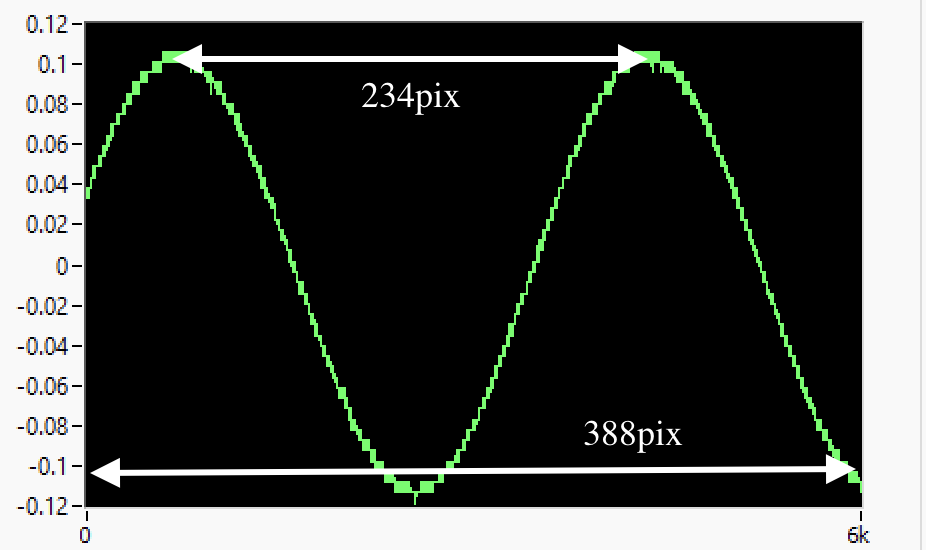
\includegraphics[width=0.6\linewidth]{figures/exp_4_2.png}
    \caption{由顯示比例推得$f_{recon.}\approx0.27591$Hz(訊號產生器頻率$f_{in}$=999.4Hz,取樣頻率$f_{s}$=998.4Hz,在6000 samples to read)}
    \label{fig:exp_4_2_crop}
\end{figure}

\clearpage


\item \textbf{比較2.5倍頻率的取樣率與接近2倍頻率取樣率的差異?為什麼?}\\
根據Fig.\ref{fig:exp_4_3},其訊號產生器頻率$f_{in}$=995.5Hz,取樣頻率$f_{s}$=2488.75Hz,在14 samples to read的顯示下,,可由畫面比例(Fig.\ref{fig:exp_4_3_crop})推得$T_{recon.}=\frac{14}{2488.75}\times\frac{146pix}{388pix}s$,也就是,$f_{recon.}\approx472.4241$Hz

\begin{figure}[h]
    \centering
    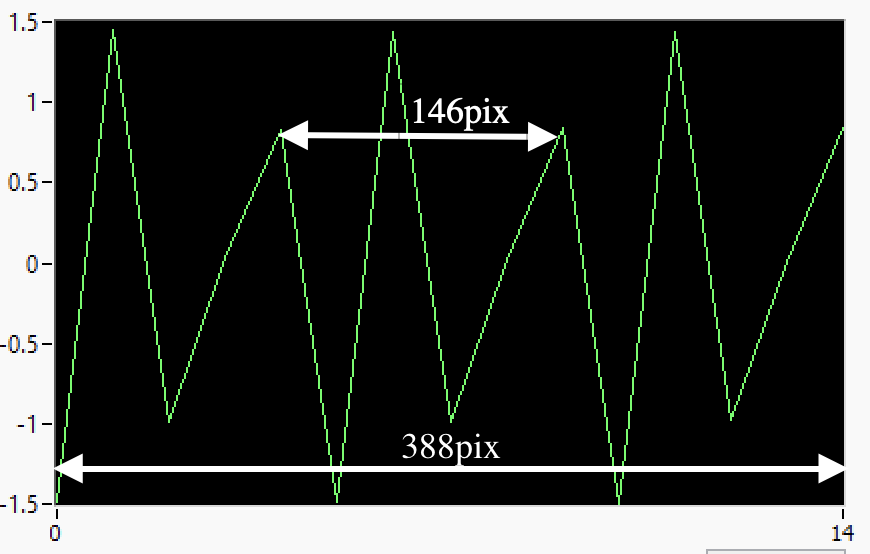
\includegraphics[width=0.6\linewidth]{figures/exp_4_3_crop.png}
    \caption{由顯示比例推得$f_{recon.}\approx472.4241$Hz(訊號產生器頻率$f_{in}$=995.5Hz,取樣頻率$f_{s}$=2488.75Hz,在14 samples to read)}
    \label{fig:exp_4_3_crop}
\end{figure}




\item \textbf{觀察不同整數倍頻率(2、3、4、5...倍)得到的圖形有甚麼不一樣?}\\

根據Fig.\ref{fig:exp_4_4_1},其訊號產生器頻率$f_{in}$=994.5Hz,取樣頻率$f_{s}$=1988.8Hz(2倍),在10 samples to read的顯示下,,可由畫面比例(Fig.\ref{fig:exp_4_4_1_crop})推得$T_{recon.}=\frac{10}{1988.8}\times\frac{87pix}{388pix}s$,也就是,$f_{recon.}\approx886.9590$Hz

\begin{figure}[h]
    \centering
    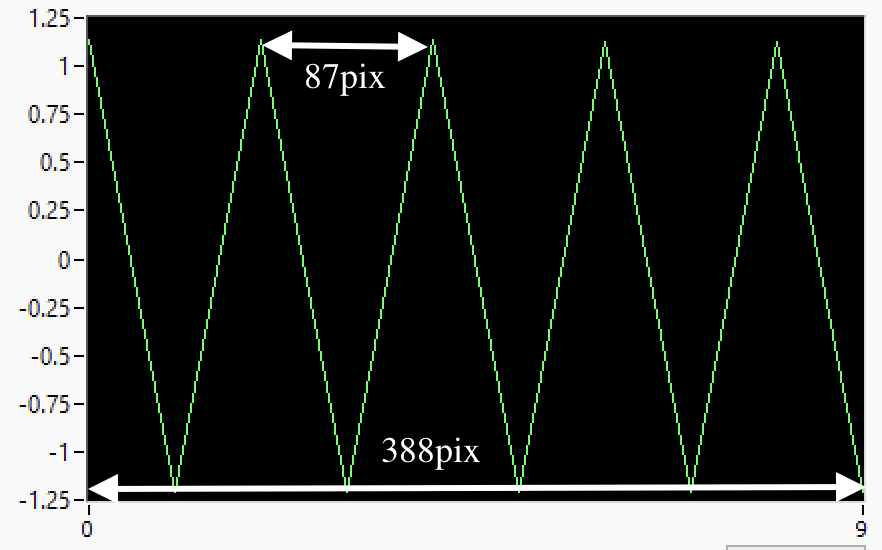
\includegraphics[width=0.6\linewidth]{figures/exp_4_4_1_crop.png}
    \caption{由顯示比例推得$f_{recon.}\approx886.9590$Hz(訊號產生器頻率$f_{in}$=994.5Hz,取樣頻率$f_{s}$=1988.8Hz(2倍),在10 samples to read)}
    \label{fig:exp_4_4_1_crop}
\end{figure}

\clearpage
根據Fig.\ref{fig:exp_4_4_2},其訊號產生器頻率$f_{in}$=994.5Hz,取樣頻率$f_{s}$=2983.5Hz(3倍),在10 samples to read的顯示下,,可由畫面比例(Fig.\ref{fig:exp_4_4_2_crop})推得$T_{recon.}=\frac{10}{2983.5}\times\frac{125pix}{390pix}s$,也就是,$f_{recon.}\approx930.8520$Hz

\begin{figure}[h]
    \centering
    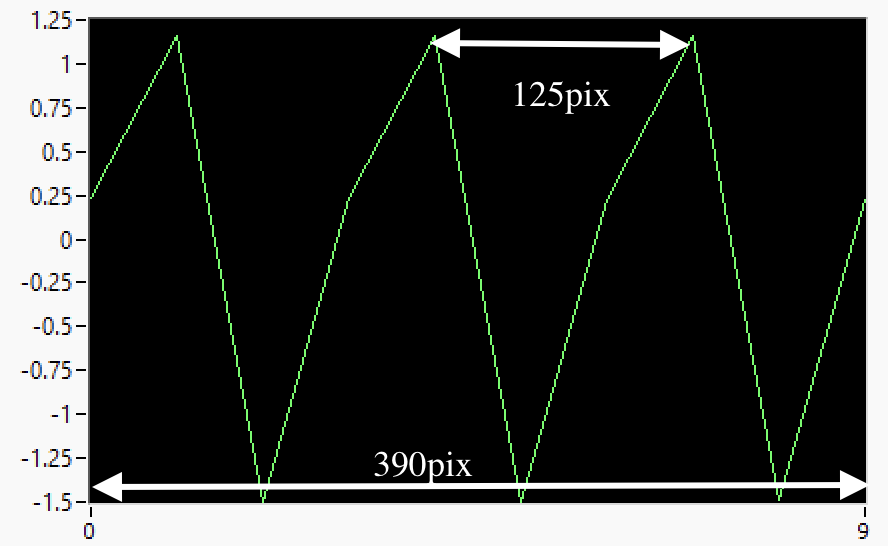
\includegraphics[width=0.6\linewidth]{figures/exp_4_4_2_crop.png}
    \caption{由顯示比例推得$f_{recon.}\approx930.8520$Hz(訊號產生器頻率$f_{in}$=994.5Hz,取樣頻率$f_{s}$=2983.5Hz(3倍),在10 samples to read)}
    \label{fig:exp_4_4_2_crop}
\end{figure}



根據Fig.\ref{fig:exp_4_4_3},其訊號產生器頻率$f_{in}$=994.5Hz,取樣頻率$f_{s}$=3977.6Hz(4倍),在10 samples to read的顯示下,,可由畫面比例(Fig.\ref{fig:exp_4_4_3_crop})推得$T_{recon.}=\frac{10}{3977.6}\times\frac{175pix}{388pix}s$,也就是,$f_{recon.}\approx881.8907$Hz

\begin{figure}[h]
    \centering
    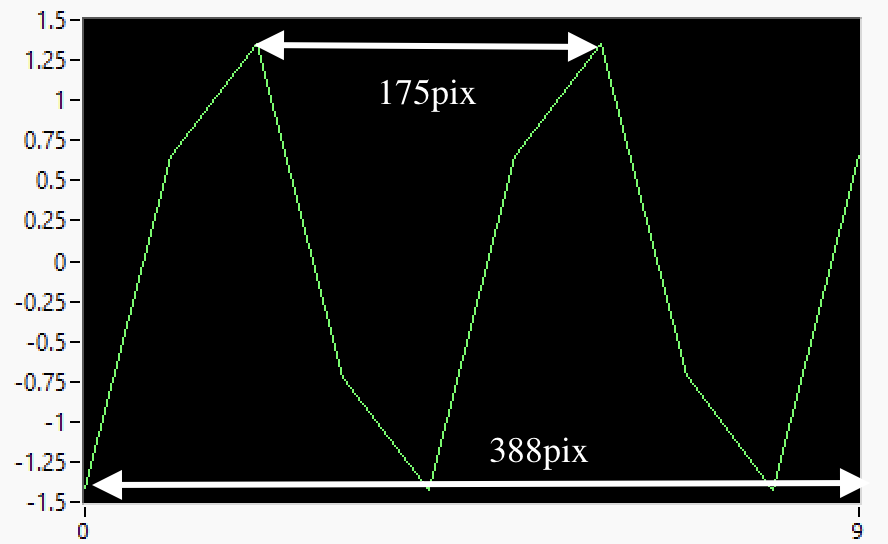
\includegraphics[width=0.6\linewidth]{figures/exp_4_4_3_crop.png}
    \caption{由顯示比例推得$f_{recon.}\approx881.8907$Hz(訊號產生器頻率$f_{in}$=994.5Hz,取樣頻率$f_{s}$=3977.6Hz(4倍),在10 samples to read)}
    \label{fig:exp_4_4_3_crop}
\end{figure}

\clearpage
根據Fig.\ref{fig:exp_4_4_4},其訊號產生器頻率$f_{in}$=994.5Hz,取樣頻率$f_{s}$=4972Hz(5倍),在10 samples to read的顯示下,,可由畫面比例(Fig.\ref{fig:exp_4_4_4_crop})推得$T_{recon.}=\frac{10}{4972}\times\frac{218pix}{394pix}s$,也就是,$f_{recon.}\approx898.6091$Hz

\begin{figure}[h]
    \centering
    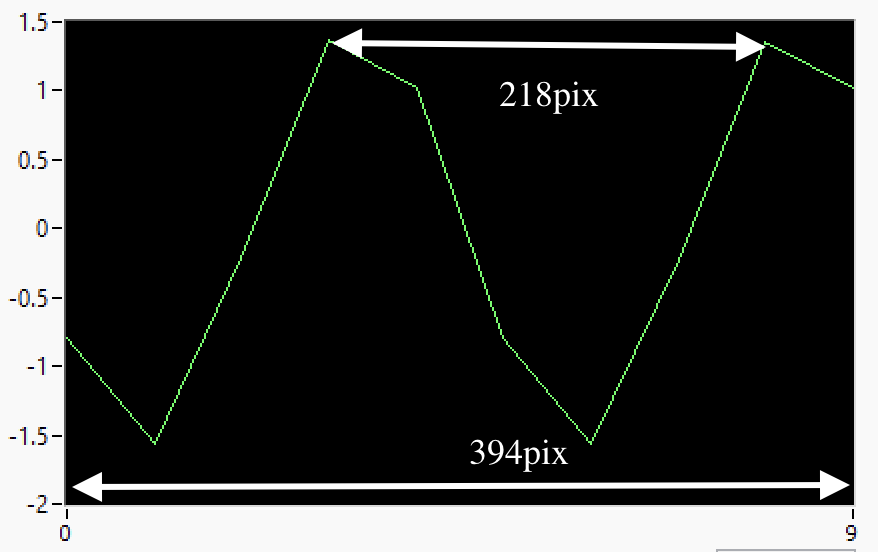
\includegraphics[width=0.6\linewidth]{figures/exp_4_4_4_crop.png}
    \caption{由顯示比例推得$f_{recon.}\approx898.6091$Hz(訊號產生器頻率$f_{in}$=994.5Hz,取樣頻率$f_{s}$=4972Hz(5倍),在10 samples to read)}
    \label{fig:exp_4_4_4_crop}
\end{figure}

根據Fig.\ref{fig:exp_4_4_5},其訊號產生器頻率$f_{in}$=994.5Hz,取樣頻率$f_{s}$=5966.4Hz(6倍),在10 samples to read的顯示下,,可由畫面比例(Fig.\ref{fig:exp_4_4_5_crop})推得$T_{recon.}=\frac{10}{5966.4}\times\frac{259pix}{395pix}s$,也就是,$f_{recon.}\approx909.9335$Hz

\begin{figure}[h]
    \centering
    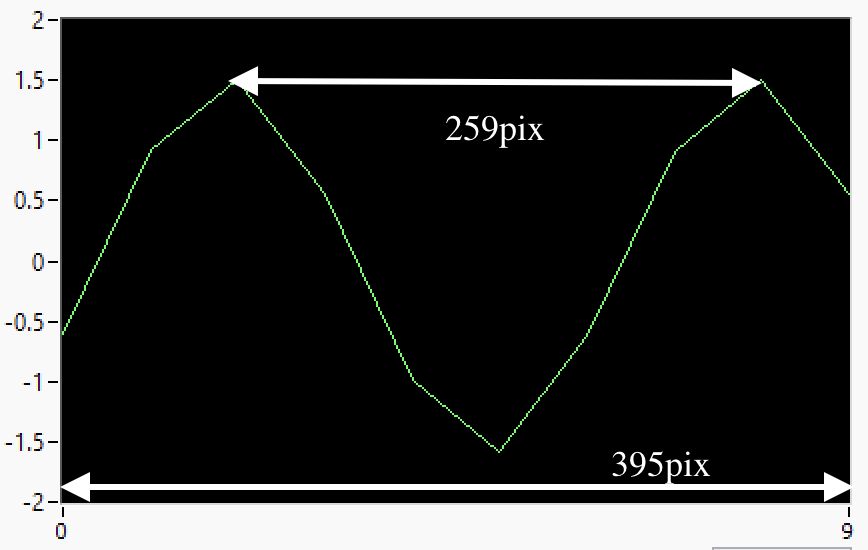
\includegraphics[width=0.6\linewidth]{figures/exp_4_4_5_crop.png}
    \caption{由顯示比例推得$f_{recon.}\approx909.9335$Hz(訊號產生器頻率$f_{in}$=994.5Hz,取樣頻率$f_{s}$=5966.4Hz(6倍),在10 samples to read)}
    \label{fig:exp_4_4_5_crop}
\end{figure}

\clearpage

根據Fig.\ref{fig:exp_4_4_6},其訊號產生器頻率$f_{in}$=994.5Hz,取樣頻率$f_{s}$=6960.8Hz(7倍),在10 samples to read的顯示下,,可由畫面比例(Fig.\ref{fig:exp_4_4_6_crop})推得$T_{recon.}=\frac{10}{6960.8}\times\frac{296pix}{392pix}s$,也就是,$f_{recon.}\approx921.8356$Hz

\begin{figure}[h]
    \centering
    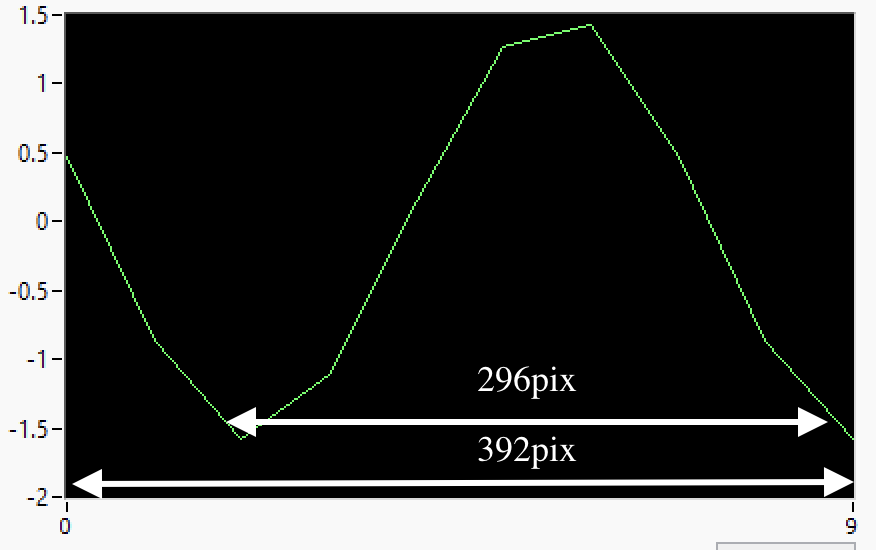
\includegraphics[width=0.6\linewidth]{figures/exp_4_4_6_crop.png}
    \caption{由顯示比例推得$f_{recon.}\approx921.8356$Hz(訊號產生器頻率$f_{in}$=994.5Hz,取樣頻率$f_{s}$=6960.8Hz(7倍),在10 samples to read)}
    \label{fig:exp_4_4_6_crop}
\end{figure}

統整上述數據分析,可得表:
\begin{center}
\begin{tabular}{c|c|c}
$f_{in}$    &   $f_{s}$ &   $f_{recon.}$\\\hline
\multicolumn{3}{c}{(Hz)}\\\hline\hline
994.5   &   1988.8($\times 2f_{in}$)  &   887.0   \\\hline
994.5   &   2983.5($\times 3f_{in}$)  &   930.9   \\\hline
994.5   &   3977.6($\times 4f_{in}$)  &   881.9   \\\hline
994.5   &   4972.0($\times 5f_{in}$)  &   898.6   \\\hline
994.5   &   5966.4($\times 6f_{in}$)  &   921.8   \\\hline
994.5   &   6960.8($\times 7f_{in}$)  &   921.8   \\\hline
\end{tabular}
\end{center}
由推算出的$f_{recon.}$,和奈奎斯特取樣定理(Sec.\ref{subsec:ny}),可推論在不同整數倍頻率\\(2、3、4、5...倍)得到的圖形大致相同,但由於訊號產生器所供給的頻率$f_{in}$無法精準控制於一固定值,因此由DAQ card取樣後的$f_{recon.}$無法與實際$f_{in}$相同。

\item \textbf{從以上觀察取樣率要幾倍以上才能獲得正確頻率?為什麼?}\\
根據實驗原理Sec.\ref{subsec:ny},和Fig.\ref{fig:exp_4_4_1_crop}-\ref{fig:exp_4_4_6_crop},取樣率$f_{s}$應大於等於2$f_{in}$。

若取樣率$f_{s}$小於2$f_{in}$,也就是undersampled,其頻譜會產生混疊(aliasing effect),使得高頻訊號會錯誤映射到較低頻率,造成失真。

\item \textbf{幾倍以上才能獲得正確振福? 為什麼?}\\

根據參考資料[3],計算振幅誤差可由:
\begin{equation*}
    Amplitude Error = 100\left(1-\frac{R}{\sqrt{1+R^2}} \right)
\end{equation*}
其中$R$ = $BW/f_{in}$,BW為是示波器頻寬。因此示波器頻寬最好要在測得訊號相關最高頻率成分的 3 到 5 倍之間,使得Amplitude Error於5\%以下。



\end{enumerate}





\section{分工內容}
\hfill

\begin{itemize}
    \item 洪瑜:練習一、三數據分析,和紀錄實驗數據
    \item 黃巧涵:PicoScope與訊號產生器操作,練習二數據分析
    \item 洪懌平:練習二、三實驗操作,練習四數據分析和回答問題
\end{itemize}


\section{參考文獻}
\hfill
\begin{enumerate}
    \item \url{https://www.youtube.com/watch?v=ahh1aIJbxdA&t=217s}
    \item \url{https://zh.wikipedia.org/zh-tw/%E6%88%B4%E7%BB%B4%E5%8D%97%E5%AE%9A%E7%90%86}
    \item \url{https://shorturl.at/y9P2a}
\end{enumerate}
    


\end{CJK}
\end{document}
